\chapter{A direct test of time reversal symmetry with neutral K mesons}
\label{chapter:test_kloe}

%
% TODO: dopisac, ze niezalezny od CP
% 

%% introductory words
Reversal of a process in time, in its most intuitive sense, means an inversion of the arrow of time so that a process of transition from state A to state B becomes a passage from B to A. In a more detailed consideration, one can note that also the states A and B may not be symmetric under the \Ts~transformation, so that the transition reversed in time is in fact $\mathcal{T}(\mathrm{A}\to\mathrm{B}) = \mathcal{T}(\mathrm{B})\to\mathcal{T}(\mathrm{A})$. In the case of spinless particles such as neutral K mesons, however, the possible particle states are in fact \Ts-symmetric so that the notion of reversing a transition between states in time remains very close to the natural understanding of \textit{``time reversal''}. The beauty of the concept of a direct test of the \Ts~symmetry therefore lies in its proximity to the commonsense intuition behind testing whether Nature is symmetric under reversal in time by comparing whether a process A$\to$B is equally likely as B$\to$A. This Chapter presents the principles of such \Ts~symmetry test using transitions of neutral kaons between strangeness and \CPs~eigenstates along with prospects for its experimental realization with the KLOE setup. A more detailed description of this measurement concept can be found in Reference~\cite{theory:bernabeu-t}.

\section{Definition of the compared processes}
As explained in Section~\ref{sec:kaons}, the state of a neutral K meson can be described either in the flavour basis, i.e.\ the basis of $\{\kaon,\akaon\}$ states of definite strangeness or in the basis of eigenstates of the \CPs~operator $\left\{\Kp,\Km\right\}$. In order to prepare a direct test of the symmetry under reversal in time, transitions between certain kaon states must be observed experimentally as well as their \Ts-conjugates obtained by an exchange of initial and final states. To this end, transitions between pure flavour and \CPs-definite neutral kaon states can be used, allowing to define a total of eight transitions as shown in \fref{fig:transitions}. As half of these processes are time-reversal conjugates of the others,
four of them are chosen as reference transitions and compared to their T-inverted counterparts.

The direct symmetry test is based on a comparison of probabilities among such process pairs, therefore four observables $R_{i}$ ($i=1,\ldots 4$) are defined as ratios of probability of each reference and its \Ts-conjugated process:
\begin{eqnarray}
  R_1(\Delta t)  = \frac{P[\kaon(0) \to \Kp(\Delta t)]}{P[\Kp(0) \to \kaon(\Delta t)]}, \label{eq:r1t}\\
  {R_2(\Delta t)}  = {\frac{P[\kaon(0) \to \Km(\Delta t)]}{P[\Km(0) \to \kaon(\Delta t)]} },\label{eq:r2t}\\
  R_3(\Delta t)  = \frac{P[\akaon(0) \to \Kp(\Delta t)]}{P[\Kp(0) \to \akaon(\Delta t)]},\label{eq:r3t} \\
  {R_4(\Delta t)}  = {\frac{P[\akaon(0) \to \Km(\Delta t)]}{P[\Km(0) \to \akaon(\Delta t)]} }.\label{eq:r4t}
\end{eqnarray}
It can be shown that such probability asymmetries must be time-dependent~\cite{theory:bernabeu-t}, therefore the above ratios are functions the time $\Delta t$ of the evolution of the kaon between given initial and final states. If invariance under reversal in time holds, all these ratios are expected to be equal to unity for any value of $\Delta t$.

\section{Principle of observation of transitions}
In an experiment, the probabilities used to define the ratios from Equations~\ref{eq:r1t}--\ref{eq:r4t} are measurable through rates of events where a given transition is observed to occur in a certain time interval $\Delta t$. Registration of such events requires identification of kaon state in two moments of its evolution, $t=0$ and $t=\Delta t$. In the latter case, final state of a transition is easily recognized by observing the kaon decay into a certain final state, where semileptonic decays are only possible for $\kaon$ and $\akaon$ and final states with two or three pions indicate that the decaying kaon was in a pure $\Kp$ or $\Km$ state, as summarized in~\tref{tab:tagging}.

Identification of an initial state for a transition must be performed in a non-destructive way in order to observe further evolution of the kaon, to which end the peculiar properties of pairs of neutral K mesons produced in certain strong decays can be employed. In the decay of a $\phi$ meson with $J^{PC}=1^{--}$ into two neutral kaons, conservation of quantum numbers by the strong interaction results in the products created in a quantum-entangled antisymmetric state which may be expressed in the flavour basis as
\begin{equation}
  \label{eq:entangled1}
  \ket{i} = \frac{1}{\sqrt{2}}\left( \ket{\kaon(+\vec{p})}\ket{\akaon(-\vec{p})} - \ket{\akaon(+\vec{p})}\ket{\kaon(-\vec{p})} \right),
\end{equation}
or equivalently with the \CPs~eigenstates as
\begin{equation}
  \label{eq:entangled2}
  \ket{i} = \frac{1}{\sqrt{2}}\left( \ket{\Kp(+\vec{p})}\ket{\Km(-\vec{p})} - \ket{\Km(+\vec{p})}\ket{\Kp(-\vec{p})} \right),
\end{equation}
where the two kaons are distinguished by the sense of their momentum in the center-of-mass reference frame. Such neutral kaon pairs, exhibiting entanglement in the genuine sense first described by Einstein, Podolsky and Rosen~\cite{Einstein:1935rr}, allow for determination of the state of a kaon without its decay by observation of an earlier decay of its entangled partner. Entanglement requires that at the moment of decay of the first of two kaons, when observed products allow to tag its state in one of the bases, the second kaon which did not decay yet must be in an orthogonal state. This state, inferred from the other kaon decay, is used as initial state of the transitions investigated in the direct \Ts~symmetry test. This principle is depicted schematically for the case of a $\akaon\to\Km$ transition in Figure~\ref{fig:principle}. As a consequence of this measurement scheme, each of the kaon transitions entering the ratios shown in Equations~\ref{eq:r1t}--\ref{eq:r4t} is identified experimentally by observation of a time-ordered pair of certain neutral kaon decays. \tref{tab:processes} summarizes the compared transitions and their experimental signatures.
%
\begin{figure}[h!]
  \centering
  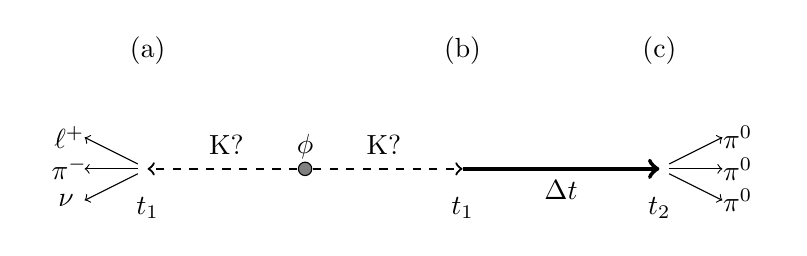
\begin{tikzpicture}[scale=1.0] %, show background rectangle]                   
    \node (first) at (-2,0){};
    \node (same) at (2,0){};
    \node (second) at (4.5,0){};
    \node[circle, inner sep=0.06cm, fill=gray,draw] at (0,0) {} node[above] {$\phi$};
    \draw[thick, dashed, ->] (0.1,0) -- (2,0);
    \draw[thick, dashed, ->] (-0.1,0) -- (-2,0);
%      
    \node at (-1,0.3) {$\mathrm{K}?$};
    \node at (1,0.3)  {$\mathrm{K}?$};
%
      \node (t12) at (2,-0.5) {$t_1$};
      \node (t11) at (-2,-0.5) {$t_1$};
      %
      \draw[black, ->] (first) -- (-2.8,0) node[] {$\pi^-\;\;\;\;$};
      \draw[black, ->] (first) -- (-2.8,0.4) node[] {$\ell^+\;\;\;\;$};
      \draw[black, ->] (first) -- (-2.8,-0.4) node[] {$\nu\:\;\;\;\;$};
      % 
      \node at (-1.7,0.7) {$\ket{\kaon}$};
      \node (decay1) at (-2,0.5) {};
      \node[above of=decay1, text width=8em, text centered] {(a)};
%      \draw[thick, red, ->] (decay1) -- (first);
      \node (decay2) at (2,0.5) {};
      \node[above of=decay2, text width=11em, text centered] {(b)};
%      \draw[thick, red, ->] (decay2) -- (same);
      \node at (2,0.7) {$\ket{\akaon}$};
      % 
      \draw[ultra thick, black, ->] (2,0) -- (4.5,0) node[midway,below] {$\Delta t$};
      % \node[star,star points=10, inner sep=0.06cm, draw, thick, fill=orange!100] at (second) {};
      \node (t21) at (4.5,-0.5) {$t_2$};
      %
      \draw[black, ->] (second) -- (5.3,0) node[] {$\;\;\;\;\pi^0$};
      \draw[black, ->] (second) -- (5.3,0.4) node[] {$\;\;\;\;\pi^0$};
      \draw[black, ->] (second) -- (5.3,-0.4) node[] {$\;\;\;\;\pi^0$};
      % 
      \node at (4.3,0.7) {$\ket{\Km}$};
      \node (decay3) at (4.5,0.5) {};
      \node[above of=decay3, text width=8em, text centered] {(c)};
%      \draw[thick, red, ->] (decay3) -- (second);
  \end{tikzpicture}
  \caption{\label{fig:principle}
    Scheme of experimental observation of a $\akaon\to\Km$ transition using quantum  entanglement of $\kaon\akaon$ pairs. Dashed arrows denote initial propagation of the entangled kaons produced in a $\phi$ decay when neither of the states is known. (a) At time $t_1$, first of the kaons undergoes a $\mathrm{K}\to \pi^- \ell^+ \nu$ decay and is identified as $\kaon$ (see~\tref{tab:tagging}). (b)~At~the same time, its entangled partner is known to be in an $\akaon$ state. (c) After further propagation, its decay into $3\pi^0$ at time $t_2$ identifies the kaon as the $\Km$ state. Thick arrow denotes thus observed $\akaon\to\Km$ process happening in time $\Delta t=t_2-t_1$.
  }
\end{figure}

It is worth noting that in the above considerations the kaon states identified by their decays into two and three pions are supposed to be pure \CPs~eigenstates $\Kp$ and $\Km$ and to be exactly orthogonal, which is crucial for the use of quantum entanglement. However, as a result of direct \CPs~violation in the neutral kaon system, the decaying states $\Ks$ and $\Kl$ as defined in Equations~\ref{eq:kskl}, are not perfectly orthogonal, with $\braket{\Ks}{\Kl}\approx \epsilon_L + \epsilon_S^*$. Therefore, the considerations described herein explicitly neglect \CPs~violation in neutral kaon decays so that:
\begin{eqnarray}
  \label{eq:cp_neglect}
  \ket{\Kp} \simeq \ket{\Ks},\\
  \ket{\Km} \simeq \ket{\Kl}.
\end{eqnarray}
It has been shown in Reference~\cite{theory:bernabeu-t} that \CPs~violation indeed does not have a substantial effect on the measurement of the asymmetric ratios defined in Equations~\ref{eq:r1t}--\ref{eq:r4t}.

\begin{table}[h]
  \centering
  \caption{\label{tab:processes}Four transitions between flavour and \CPs~eigenstates available in the neutral kaon system and their time-reversal conjugates with initial and final states exchanged. Each of the listed processes is experimentally identified by a time-ordered pair of kaon decays into final states indicated in parentheses. }
    \begin{tabular}{lllll}
      \toprule
      No. &  \multicolumn{2}{c}{Transition}   & \multicolumn{2}{c}{\Ts-conjugate}  \\
      \midrule
      1 &  $\kaon \to \Kp$ & $(\pi^+\ell^-\bar{\nu},\pi\pi)$ & $\Kp \to \kaon$ & $(3\pi^0, \pi^-\ell^+\nu)$ \\
      2 &  $\kaon \to \Km$ & $(\pi^+\ell^-\bar{\nu}, 3\pi^0)$ & $\Km \to \kaon$ & $(\pi\pi,\pi^-\ell^+\nu)$  \\
      3 &  $\akaon \to \Kp$ & $(\pi^-\ell^+\nu,\pi\pi)$ & $\Kp \to \akaon$ & $(3\pi^0, \pi^+\ell^-\bar{\nu})$ \\
      4 &  $\akaon \to \Km$ & $(\pi^-\ell^+\nu,3\pi^0)$ & $\Km \to \akaon$ & $(\pi\pi, \pi^+\ell^-\bar{\nu})$ \\
      \bottomrule
    \end{tabular}
\end{table}

%TODO: sprawdzic czy mathrm w dsdq bylo w poprzednim rodziale
A second assumption which is taken in the direct test of the symmetry under time reversal, is the validity of the $\Delta S=\Delta Q$ rule in semileptonic kaon decays, which is employed in identification of flavour states of neutral kaons. This rule, however, has been thoroughly tested to date and no evidence exists for its violation~\cite{pdg2016}.

\section{Observables of the test}\label{sec:observables}
The principle of observation of neutral kaon transitions between flavour and \CPs~states using quantum entanglement requires that two kaon decays are observed in a single \mbox{$\phi\to\kaon\akaon$} event in order to identify a certain transition, and that their proper decay times are determined precisely to measure $\Delta t$. Each of the transitions listed in~\tref{tab:processes} is therefore identified by registration of a time-ordered pair of specific neutral kaon decays, indicated next to the transitions in the table. It should be emphasized that the first decay in each pair corresponds to an entangled partner of the kaon whose transition if observed and thus tags a state opposite to the initial one in the transition of interest.

Directly observable values comprise distributions of rates of events $I(f_1,f_2;\Delta t)$ characterized by two kaon decays into final states $f_1$ and $f_2$ as a function of the time interval $\Delta t$ between both decays measured in the kaons' proper reference frames. For the case of neutral K meson pairs produced in $\phi$ decays, the theoretical \Ts-asymmetric ratios defined in Equations~\ref{eq:r1t}--\ref{eq:r4t} are linked with the experimantally-measurable ratios of decay rates $R^{exp}$ defined in the following way:
  \begin{eqnarray}
    R_1^{exp}(\Delta t) & = \frac{\mathrm{I}(\pi^+\ell^-\bar{\nu},\pi\pi;\Delta t)}{\mathrm{I}(3\pi^0,\pi^-\ell^+\nu;\Delta t)} {  = R_1(\Delta t)\times  \frac{C(\pi^+\ell^-\bar{\nu},\pi\pi)}{C(3\pi^0,\pi^-\ell^+\nu)}},  \label{eq:r1e}\\
    {R_2^{exp}(\Delta t)} & = \frac{\mathrm{I}(\pi^+\ell^-\bar{\nu},3\pi^0;\Delta t)}{\mathrm{I}(\pi\pi,\pi^-\ell^+\nu;\Delta t)} {  = R_2(\Delta t) \times \frac{C(\pi^+\ell^-\bar{\nu},3\pi^0)}{C(\pi\pi,\pi^-\ell^+\nu)}}, \label{eq:r2e} \label{eq:r2def}\\
    R_3^{exp}(\Delta t) & = \frac{\mathrm{I}(\pi^-\ell^+\nu,\pi\pi;\Delta t)}{\mathrm{I}(3\pi^0,\pi^+\ell^-\bar{\nu};\Delta t)} {  = R_3(\Delta t) \times \frac{C(\pi^-\ell^+\nu,\pi\pi)}{C(3\pi^0,\pi^+\ell^-\bar{\nu})}}, \label{eq:r3e}\\
    {R_4^{exp}(\Delta t)} & = \frac{\mathrm{I}(\pi^-\ell^+\nu,3\pi^0;\Delta t)}{\mathrm{I}(\pi\pi,\pi^+\ell^-\bar{\nu};\Delta t)} {  = R_4(\Delta t) \times \frac{C(\pi^-\ell^+\nu,3\pi^0)}{C(\pi\pi,\pi^+\ell^-\bar{\nu})}} \label{eq:r4e} \label{eq:r4def},
  \end{eqnarray}
  where $C(f_1,f_2)$ denote coefficients dependent on transition amplitudes of neutral kaons to particular final states $f_1$ and $f_2$~\cite{theory:bernabeu-t}. It can be shown that these coefficients are symmetric with respect to an interchange of final states of the first and second decay, i.e.:
  \begin{equation}
    \label{eq:c_sym}
    C(f_1,f_2) = C(f_2,f_1).
  \end{equation}

Although all of the experimental ratios $R^{exp}_{1}$--$R^{exp}_{4}$ use independent physical processes, one can note that they are pairwise equivalent to their inverses if the order of observed decays is reversed. Therefore, using the symmetry of the $C$ coefficients from \eref{eq:c_sym}, one can express possibilities by only two \Ts-asymmetric ratios if the time difference between kaon decays is allowed to be negative:
\begin{eqnarray}
  R_2^{exp}({-\Delta t}) & = \left({R_3^{exp}(\Delta t)}\right)^{-1}, \\
  R_4^{exp}({-\Delta t}) & = \left({R_1^{exp}(\Delta t)}\right)^{-1}.
\end{eqnarray}

The above observation makes it sufficient to consider only two out of four ratios if any order of the kaon decays is allowed so that $\Delta t \in (-\infty,+\infty)$. In the further considerations only the $R_2$ and $R_4$ will thus be included, following the convention used in Ref.~\cite{theory:bernabeu-t}. 

\begin{figure}[htb]
  \centering
  \includegraphics[width=0.6\textwidth]{Chapter4_test_kloe/img/largeDt}
  \caption{\label{fig:strategy}
    Expected dependence of the observable asymmetric ratios  $R^{exp}_2(\Delta t)$ and $R^{exp}_4(\Delta t)$ on the time difference between kaon decays in presence of \Ts~violation.
    Symmetry violation effects can be sought either as significant $\Delta t$ dependence for small and negative values of $\Delta t$ or as deviation of the asymptotic value $R(\Delta t \gg \tau_{S})$ from unity.
    Figure adapted from~\cite{theory:bernabeu-t}.
  }
\end{figure}

\section{Possible measurement strategies}\label{sec:strategies}
The observable double decay rate ratios defined in Equations~\ref{eq:r2e} and~\ref{eq:r4e} in case of violation of the symmetry under reversal in time are expected to depend on the kaons' decay time difference $\Delta t$ as shown on the plots in~\fref{fig:strategy}. For small time differences and especially for $\Delta t < 0$ one can search for effects of \Ts~violation manifested in the form of structures in the $\Delta t$ dependence of the $R^{exp}_2(\Delta t)$ and $R^{exp}_4(\Delta t)$ ratios. Authors of Reference~\cite{theory:bernabeu-t} have shown that significant deviations from constant value are expected in case of broken symmetry (see \fref{fig:strategy}). On the other hand, in the region of $\Delta t \gg \tau_{S}$ (where $\tau_S$ denotes $\Ks$ lifetime) the ratios are expected to reach a constant asymptotic level. Therefore, a measurement of the asymptotic level of $R^{exp}_2(\Delta t)$ and $R^{exp}_4(\Delta t)$ constitutes another available strategy to search for breaking of he \Ts~symmetry. In agreement with the commonsense expectation, any deviation of the theoretical ratios $R_2$ and $R_4$ (extracted from $R^{exp}_2$ and $R^{exp}_4$ using the respective $C(f_1,f_2)$ factors as in Equations~\ref{eq:r2e} and~\ref{eq:r4e}) from unity would be an indication of violated \Ts~symmetry. It can be shown that such deviations are proportional to the real part of the \Ts-violating $\epsilon$ parameter (see Equations~\ref{eq:epsilon_delta} and~\ref{eq:kabir_epsilon})~\cite{theory:bernabeu-t}:
\begin{equation}
  \begin{aligned}
    \label{eq:theor_deviations}
    & R_2(\Delta t \gg \tau_{S}) \simeq 1-4\Re\epsilon, \\
    & R_4(\Delta t \gg \tau_{S}) \simeq 1+4\Re\epsilon.
  \end{aligned}
\end{equation}

The first of the aforementioned measurement strategies requires collection of a large number of double kaon decay events within a small range of decay time differences, where additionally the negative $\Delta t$ region would be populated by events where first kaon decayed into three neutral pions and the second one into the $\pi\ell\nu$ final state.

However, the probability of the long-lived neutral kaon decaying before its short-lived partner is small (at the level below \SI{1}{\percent}) and a decay of $\Ks$ into three neutral pions is a \CPs-violating decay whose branching ratio is below 2.6$\times 10^{-8}$ by the searches performed so far, which found no candidate events~\cite{Babusci:2013tr}.
%Practically, due to large difference of lifetimes between $\Ks$ and $\Kl$ this would have to result mostly from $\Ks\to 3\pi^0$ and
As a consequence, observation of the $R_{2(4)}^{exp}$ region for small and negative $\Delta t$ would require very high statistics and is thus not feasible with the KLOE detector at the DA$\Phi$NE collider.
Moreover, this experimental approach would require reaching a resolution of kaon decay times difference sufficient to observe the structures in $\Delta t$ dependence of $R_{2(4)}^{exp}$.


Conversely, the test exploiting the asymptotic region of large time differences can be performed with KLOE and DA$\Phi$NE as large numbers of events are expected for $\Delta t \gg \tau_{S}$ and as such measurement would comprise averaging over a broad range of time differences. This is an advantage of KLOE, whose size allows it to capture double decay  events with $\Delta t$ up to almost 400 $\tau_{S}$. Moreover, kaons' decay time reconstruction is not required at a level as precise as in the case of searching for structures in the time dependence. Thus in case of this measurement, resolution of the $\Kl\to 3\pi^0$ decay is not a limiting factor despite challenges related to its reconstruction which will be discussed in Chapter~\ref{chapter:gps}.

Application of the test of symmetry under reversal in time by determination of the asymptotic values of the $R^{exp}_2(\Delta t)$ and $R^{exp}_4(\Delta t)$ ratios is one of the goals of the KLOE-2 experiment and is expected to yield a statistically significant result using an integrated luminosity of the order of 5 fb$^{-1}$~\cite{theory:bernabeu-t}. In the time when this data is being collected, data reconstruction and analysis methods required for this test were devised using a dataset of the KLOE experiment. Their preparation and application to KLOE data constitute a major part of the work reported on in this Thesis. 

\section{Determination of the constant coefficient in asymmetric ratios}\label{sec:d_determination}
As shown in Equations~\ref{eq:r1e}--\ref{eq:r4e}, the experimentally-observable ratios $R^{exp}_{1-4}$ are linked to the theoretical ratios of certain transitions' probability with proportionality constants dependent on particular kaon decays identifying the transitions used to define the ratios. 

\begin{eqnarray}
 \frac{C(\pi^+\ell^-\bar{\nu},3\pi^0)}{C(\pi\pi,\pi^-\ell^+\nu)} = \left|\frac{\expval{\pi^+\ell^-\bar{\nu}|\mathbb{T}|\akaon}\expval{3\pi^0|\mathbb{T}|\Km}}{\expval{\pi^-\ell^+\nu|\mathbb{T}|\kaon}\expval{\pi\pi|\mathbb{T}|\Kp}}\right|^2,\\  
  \frac{C(\pi^-\ell^+\nu,3\pi^0)}{C(\pi\pi,\pi^+\ell^-\bar{\nu})} = \left|\frac{\expval{\pi^-\ell^+\nu|\mathbb{T}|\kaon}\expval{3\pi^0|\mathbb{T}|\Km}}{\expval{\pi^+\ell^-\bar{\nu}|\mathbb{T}|\akaon}\expval{\pi\pi|\mathbb{T}|\Kp}}\right|^2,
\end{eqnarray}
where $\mathbb{T}$ denotes the transition matrix of the neutral kaon system.

If \CPTs~violating effects in semileptonic decays of neutral kaons are not allowed (which indeed have not been observed to date), the amplitudes $\expval{\pi^+\ell^-\bar{\nu}|T|\akaon}$ and $\expval{\pi^-\ell^+\nu|T|\kaon}$ are equal and both of the above coefficients reduce to the same value which will be referred to as the $D$ coefficient in further considerations:
\begin{equation}
 D \equiv \frac{C(\pi^+\ell^-\bar{\nu},3\pi^0)}{C(\pi\pi,\pi^-\ell^+\nu)} = \frac{C(\pi^-\ell^+\nu,3\pi^0)}{C(\pi\pi,\pi^+\ell^-\bar{\nu})} =  \left|\frac{\expval{3\pi^0|\mathbb{T}|\Km}}{\expval{\pi\pi|\mathbb{T}|\Kp}}\right|^2.
  \label{eq:c_coeff_1}
\end{equation}
The decay probabilities which define the above can be expressed with branching fractions of these decays and the respective kaon lifetimes $\tau_S$ and $\tau_L$ of the short and long-lived kaons, respectively. If additionally the \CPs~violation in neutral kaon decays is neglected as in \eref{eq:cp_neglect}, the coefficient from~\ref{eq:c_coeff_1} can be completely expressed in terms of experimentally-measured quantities:
\begin{equation}
  \label{eq:D}
  D \equiv \left|\frac{\expval{3\pi^0|\mathbb{T}|\Km}}{\expval{\pi\pi|\mathbb{T}|\Kp}}\right|^2 \simeq \frac{\left|\expval{3\pi^0|\mathbb{T}|\Kl}\right|^2}{\left|\expval{\pi\pi|\mathbb{T}|\Ks}\right|^2} = \frac{\text{BR}(\Kl\to 3\pi^0)\Gamma_L}{\text{BR}(\Ks\to\pi\pi)\Gamma_S} = \frac{\text{BR}(\Kl\to 3\pi^0)\tau_S}{\text{BR}(\Ks\to\pi\pi)\tau_L}.
\end{equation}

Determination of the $D$ parameter value is required in order to extract the ratios of kaon transition probabilities $R_2(\Delta t)$ and $R_4(\Delta t)$ from the observable ratios of decay rates defined in equations~\ref{eq:r2e} and~\ref{eq:r4e}:
\begin{eqnarray}
  R_2(\Delta t) = R^{exp}_2(\Delta t) / D, \\
  R_4(\Delta t) = R^{exp}_4(\Delta t) / D.
\end{eqnarray}

As the four values entering the calculation of $D$ (see \eref{eq:D}), one may choose either averages of available measurements, e.g.\ the ones extracted by the Particle Data Group (PDG)~\cite{pdg2016} or results of measurements performed by the same experimental system used for the T symmetry test. In case of the KLOE experiment, all the quantities of interest have been already measured with the same setup, thus allowing for a self-contained determination of the $R_2$ and $R_4$ asymmetries. It should also be noted that the results of KLOE measurements are in most cases (except the lifetime of $\Ks$) the most precise results entering the PDG averages. The value of $\Kl$ branching ratio for $\Kl\to 3\pi^0$ was determined in a comprehensive study of dominant $\Kl$ decays performed by the KLOE experiment in 2006~\cite{kloe_kl3pi0_br}. Although this study involved a fit which yielded the $\Kl$ lifetime, for the following calculations a result of a direct measurement, also conducted by KLOE~\cite{kloe_kl_lifetime}, was used. Similarly, for the values of $\Ks\to\pi^+\pi^-$ branching ratio and lifetime, results of high precision KLOE measurements~\cite{kloe_kspipi_br,kloe_ks_lifetime} were taken.

\tref{tab:D_inputs} presents a comparison of the values of the relevant branching ratios and lifetimes as determined by the KLOE experiment and as the PDG averages, as well as the D parameter values resulting from calculations based on these inputs.

\begin{table}[h!]
  \centering
  \caption{Quantities entering the calculation of the D parameter determined by KLOE and by PDG\@. Last row contains the values of D evaluated with each set.}\label{tab:D_inputs}
  \begin{tabular}[h!]{cS[table-format=2.12]S[table-format=2.12]}
    \toprule 
    & {KLOE measurement~\cite{kloe_kl3pi0_br,kloe_kspipi_br,kloe_kl_lifetime,kloe_ks_lifetime}} & {PDG average~\cite{pdg2016}} \\
    \midrule
    BR($\Kl\to 3\pi^0$) & 0.1997(20) & 0.1969(26) \\
    BR($\Ks\to \pi\pi$) & 0.6919(51) & 0.6920(5) \\
    $\tau_L$ [ns] & 50.92(30) & 50.99(21) \\
    $\tau_S$ [ps] & 89.562(52)  & 89.54(4) \\
    \midrule
    D & {0.5076(59)$\times 10^{-3}$} & {0.4998(69)$\times 10^{-3}$} \\
    \bottomrule
  \end{tabular}
\end{table}

As the values of the D constant parameter calculated using KLOE measurements and world averages from PDG presented in~\tref{tab:D_inputs} are consistent within their uncertainties, in the following considerations the D value obtained solely with KLOE results
\begin{equation}
  \label{eq:D_kloe}
  D = \frac{\text{BR}(\Kl\to 3\pi^0)\tau_S}{\text{BR}(\Ks\to\pi\pi)\tau_L} = 0.5076(59)\times 10^{-3},
\end{equation}
will be used in order allow for a self-contained KLOE determination of the \Ts-asymmetric observables.




%%%Local Variables:
%%% TeX-master: "../main"
%%% End:
